\documentclass{article}%
\usepackage[T1]{fontenc}%
\usepackage[utf8]{inputenc}%
\usepackage{lmodern}%
\usepackage{textcomp}%
\usepackage{lastpage}%
\usepackage{geometry}%
\geometry{left=3cm,right=3cm,bottom=2cm,top=1cm}%
\usepackage[russian]{babel}%
\usepackage{amsmath}%
\usepackage{amssymb}%
\usepackage{amsfonts}%
\usepackage{mathtext}%
\usepackage{graphicx}%
%
%
%
\begin{document}%
\normalsize%
\begin{center}%
.\\%
\vspace{12cm}%
\textbf{Лабораторная работа № 3.01: Изучение электростатического поля методом моделирования}%
\end{center}%
\begin{center}%
Исхаков Камиль Фархатович%
\end{center}%
\begin{center}%
\today%
\end{center}%
\newpage%
\section{Основные формулы:}%
\label{sec:}%

%
Средняя напряженность между двумя точками, лежащими на однойсиловой линии:\begin{displaymath}\langle E_{12} \rangle= \frac{\phi_1-\phi_2}{l_{12}}\end{displaymath}%
\newline%
где $\phi_1, \phi_2$ – потенциалы в выбранных точках, а $l_{12}$ – расстояния между данными точками%
\newline%
Поверхностная плотность зарядов проводника:\begin{displaymath}\sigma' = -\epsilon_0 \frac{\Delta \phi}{\Delta l_n}\end{displaymath}%
\newline%
где $\epsilon_0$ – постоянная электрическая постоянная, $\Delta \phi$– изменение потенциала при смещении на малое расстояние $\Delta l_n$по нормали к поверхности проводника%
\newline%
\section{Расчеты:}%
\label{sec:}%

%
$E_{\text{центра(16 10)}} = \frac{\phi_1-\phi_2}{l_{12}} = \frac{2}{0.162-0.100} = $33.333%
\newline%
$E_{\text{окр+}} = \frac{\phi_1-\phi_2}{l_{12}} = \frac{12.01-11.25}{0.286-0.265} = $36.19%
\newline%
Расчет погрешностей измерений:\begin{displaymath}\Delta E = \sqrt{\left(\frac{2\cdot \Delta \phi_i}{3 l}\right)^2+\left(\frac{2(\phi_2-\phi_1)\cdot \Delta l_i}{3 l^2}\right)^2}\end{displaymath}%
\newline%
$\Delta E_{\text{центра(16 10)}}$ = 1.2 В%
\newline%
$\Delta E_{\text{окр+}}$ = 3.4 В%
\newline%
$\sigma'_{+} = - \epsilon_0 \frac{\Delta \phi}{\Delta l_n} $= -3.203 В/м%
\newline%
$\sigma'_{-} = - \epsilon_0 \frac{\Delta \phi}{\Delta l_n} $= -4.383 В/м%
\newline%


\begin{figure}[h!]%
\centering%
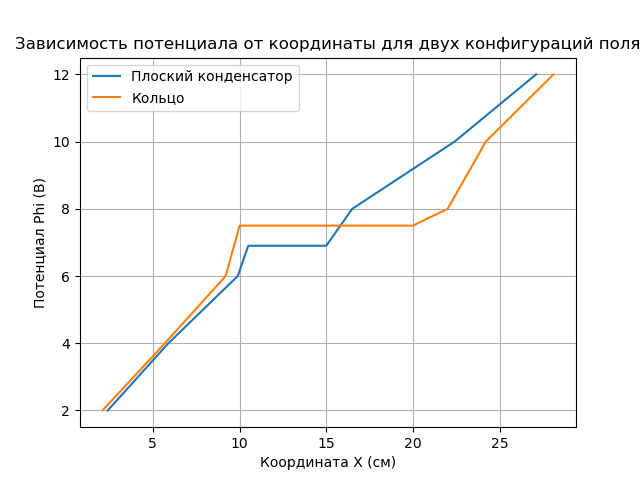
\includegraphics[width=350px]{2_potentials.png}%
\newpage%
\end{figure}

%


\begin{figure}[h!]%
\centering%
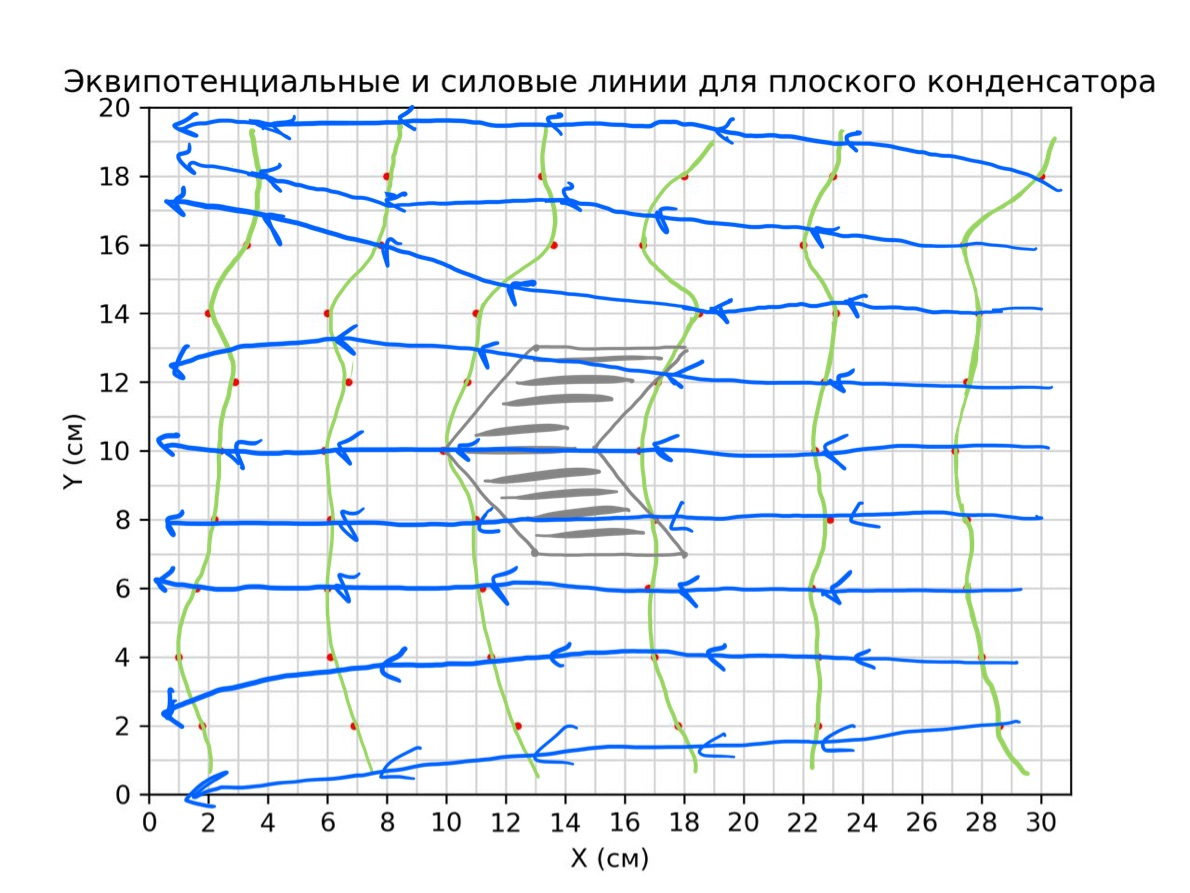
\includegraphics[width=350px]{potential_field.jpg}%
\end{figure}

%
Зеленые линии – эквипотенциальные линии; Синие линии – силовые линии.%
\newline%
\section{Выводы}%
\label{sec:}%

%
В результате выполнения лабораторной работыбыло смоделировано электрическое поле с помощью эквипотенциальных поверхностей. Стоит отметить, что верхняя часть смоделированного поля в последнем рисунке искривлена сильнее, чем нижняя. Это может быть связано с тем, что источник питания был расположен как раз ближе к верхней половине установки. Также искривления могли появиться из-за того, что недистиллированная вода могла неравномерно покрывать установку, вследствие чего одна из сторон источников питания была менее погружена другой. \\ На графике зависимости потенциала $\phi$ от икса для кольца и плоского конденсатора видно плоское плато, которое соответствует значению напряженности конденсатора и кольца (и области, заключенной внутри кольца). Причем для конденсатора характерно, что в окрестности кончика стрелки значение потенциала растет более быстро, чем в хвостике. Это соответствует действительности, поскольку количество зарядов на кончике будет больше, чем в самом конце. Расчитанные погрешности не имеют особых всплесков.%
\newline%
\end{document}